


\documentclass[a4paper]{article}

\usepackage[utf8]{inputenc}
\usepackage[french]{babel}
\usepackage{graphicx}
\graphicspath{{./img/}}
\usepackage{amsmath, amssymb}
\usepackage[left=3cm,right=3cm,top=2cm,bottom=2cm]{geometry}
\usepackage{url}
\usepackage{listings}


\usepackage[french]{babel}
\title{TP n°1 : Entropies discrète et continue, information mutuelle}
\author{Aarab Wassim - Dlimi Mohammed - Ettaki Mohammed Amine}
\date{Décembre 2023}



\begin{document}
\maketitle
\tableofcontents
\newpage
%exo 1 :
\section{Lien entre entropie discrète et continue}


\newpage

%exo 2 Partie 1:
\section{Loi gaussienne}
\subsection{Loi gaussienne univariée.}
on considère maintenant une variable aléatoire réelle $X$ qui suit une loi gaussienne de moyenne $\mu$ et de variance $\sigma^{2}$ (ie. $X \sim \mathcal{N}(\mu, \sigma^{2}))$, on veut maintenant vérifier numériquement le résultat théorique obtenu précédemment pour une variable qui suit une loi gaussienne. Il suffit donc de considérer un nombre très grand de réalisations différentes de $X$ notées $x_i$ pour qu'on puisse définir $X_{\Delta}$ avec un $\Delta$ très petit, car plus le nombre des $x_i$ qu'on choisit est grand plus que la distance entre ses éléments qui est égale à $\Delta$ est petite. On choisit par exemple $n=10000$ réalisations.\\
Pour vérifier maintenant numériquement que la densité de cette loi est bien $f_{X}=\frac{1}{\sigma\sqrt{2\pi}}\exp\left(-\frac{(x-\mu)^{2}}{2\sigma^2}\right)$, on trace l'histogramme de ces $n$ réalisations $x_{i}$ d'une aire normalisée à 1 et la densité $f_{X}$ dans une même figure. On trouve la figure ci-dessous.

\begin{figure}[h]
  \centering
  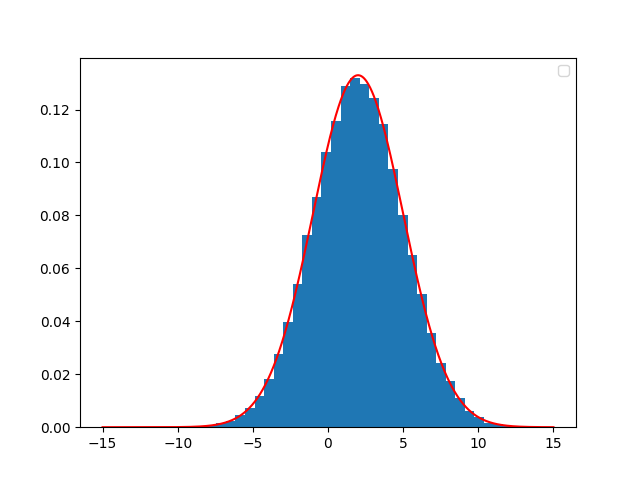
\includegraphics[width=0.8\textwidth]{Figure_1.png}
  \caption{histogramme-densité}
%  \label{hist}
\end{figure}
ceci prouve que la densité de $X$ est bien $f_X$ puisque les deux graphes sont compatibles,il nous reste maintenant à démontrer le résultat
pour se faire,on calcule numériquement $\mathbb{H}(X_\Delta)+\log(\Delta)\underset{\Delta \rightarrow 0}{\rightarrow}\mathbb{H}(X)$ à l'aide du code python fourni en annexe,et en testant on trouve la valeur $-4.092594418520442$
\newpage

%exo 2 Partie 2:
\subsection{Loi gaussienne multivariée.}
\newpage

%exo3 : 
\section{Analyse de données}

\appendix
\section{Annexe A}
\begin{figure}[h]
  \centering
  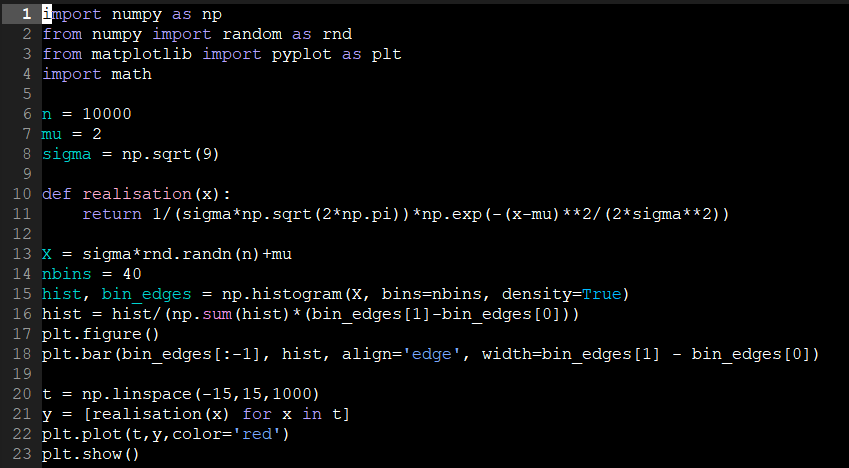
\includegraphics[width=0.8\textwidth]{1.png}
  \caption{python histogramme-densité}
%  \label{hist}
\end{figure}

\section{Annexe B}
\begin{figure}[h]
  \centering
  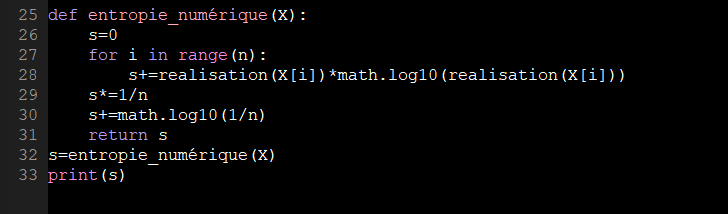
\includegraphics[width=0.8\textwidth]{2.png}
  \caption{val num}
%  \label{hist}
\end{figure}

\end{document}
